\documentclass{article}

\usepackage{geometry}[
	a4paper,
	left=3cm,
	right=2.5cm,
	top=2cm,
	bottom=2cm,
]

\usepackage{fontspec}
\usepackage{expex}
\NewCommandCopy{\expexgla}{\gla}
\usepackage{unicode-math}
\AtBeginDocument{\RenewCommandCopy{\gla}{\expexgla}}

\setmainfont{SourceSans3}[
	Extension={.ttf},
	Path=./config/fonts/,
	UprightFont={*-Regular},
	ItalicFont={*-Italic},
	BoldFont={*-Bold},
	BoldItalicFont={*-BoldItalic},
	Numbers=OldStyle,
	Kerning=On,
	Ligatures=Common,
]

%\setmathfont{LibertinusMath}[
%	Extension={.otf},
%	Path=./config/fonts/,
%	Scale=1
%]

\usepackage{graphicx}
\usepackage[all]{nowidow}

\usepackage{fancyhdr}
\fancyhf{} %clears the default

% \renewcommand{\headrulewidth}{0pt}
\fancyfoot[C]{\thepage}

%%% SECTION FORMATTING
\usepackage{titlesec}

\newcommand{\marginsecnumber}[1]{%
	\makebox[0pt][r]{#1\hspace{1em}}%
}

\titleformat{\section}[display]
{\filcenter\bfseries}
{\thesection}
{0pt}
{}

\titleformat{\subsection}[runin]
{\bfseries}
{\marginsecnumber\thesubsection}
{0pt}
{}
[.]

\titleformat{\subsubsection}[runin]
{\bfseries}
{\marginsecnumber\thesubsubsection}
{0pt}
{}






\usepackage{tabularray}
\UseTblrLibrary{booktabs}
\DefTblrTemplate{head}{default}{} %remove table head
\DefTblrTemplate{contfoot-text}{default}{\footnotesize{\emph{Cont.}}}
\DefTblrTemplate{note-tag}{default}{\rmfamily{\textsuperscript{\InsertTblrNoteTag}}}
\DefTblrTemplate{note-text}{default}{\small{\InsertTblrNoteText}}

\SetTblrOuter{long}

\usepackage[protrusion=true,expansion]{microtype}
\linespread{1.5}

\usepackage{graphicx} 
\usepackage{tikz}
\usetikzlibrary{positioning,calc}

\usepackage{subcaption}
\captionsetup{
   font={footnotesize},
width=0.8\textwidth,
}

%\usepackage{showframe}

\newcommand{\todo}{\marginpar{\sc{todo}}}

%%%Glossary commands
\newcommand{\dic}[3]{\textbf{#1} {\textsc{#2}} #3 \\}

\title{Krewi}
\author{seven vulpa}

\begin{document}
\maketitle

% \section{Introduction}%
\subsection{General background}%

Krewi is one of the chief languages spoken by people who live in the surrounding of Kyeuwal Estuary, one of the major civilizations of the region of Kredan. It is spoken at the heart of Kyehay region at the mouth of the estuary and the surrounding regions, alongside many small pockets of settlements set up by various early endeavors of colonization. The regions eastward, namely following the northern coast of Kyeuwal, are predominantly populated by Bincaruw speaking people. Following the coast even further will land into settlements which populated by Hiran people speaking many of Ceurra, or peninsular, languages, which are the languages used to be spoken at the breadth of the land. Meanwhile, the regions southward, namely following the southern coast of Kyeuwal, are predominantly populated by people speaking Cruhanya language, particularly along the riverbanks of Kyalaw and Ghildar.




\section{Phonology}%

\subsection{Consonant}%
Krewi consonants are divided into 11 contrastive units as depicted in the matrix provided below. Phonemes in brackets are borrowed-origin.

\begin{longtblr}[
		halign = c,
	]{
		rowhead = 1,
		vline{2} = {0.5pt},
		hline{2} = {0.5pt}
	}
	\toprule[1pt]
	                   & \small{labial} & \small{lingual (tip)} & \small{lingual (dorsum)} & \small{glottal} \\
	\small{nasal}      & m              & n                     &                          &                 \\
	\small{obstruents} &                & d dz                  & (dʒ)                     & x ħ (k)         \\
	\small{emphatics}  &                & ts                    & ɟʝ (tɕ)                  & kʷ kʲ           \\
	\small{continuant} & w [w ʝʷ]       & l r                   & j [j ɟ]                  &                 \\
	\bottomrule[1pt]
\end{longtblr}

Observed allophones are as follows.

\begin{itemize}
	\item Nasal /n/ can be further analyzed into two phonemes. The onset /n/ is a fairly stable phoneme which has no allophone. Meanwhile, coda /n/ allophones surface homorganically depending on the context. Coda /n/ shift the articulatory point to match the next, usually less sonorous, onset. Such phenomenon are, namely, dorsal nasal (e.g. \mbox{ɣəɲ.ɟaj}) and glottal nasal (e.g \mbox{tsɤŋ.ɡaw}). In some cases, final /n/ may surfaces the pausal form derived from the retracted point of the onset (e.g. \mbox{wɛ.raɲː}).
	\item Native obstruents, in exception of /ħ/, realize in many degree of strength. Beside the condition whichever plain [d dz x] occur, tense [t k] are only realized before laterals [l r]. Lax [ɾ z h\textasciitilde Ø] are only realized in intervocalic conditions. Labialized [tʷ ɡʷ] are only realized in the stop + semivowel [w] sequence. Meanwhile, the presence of the semivowel [j] turns obstruents into supra-tense emphatics [ɟʝ kʲ], but despite the relatedness, they fall into different phonemes.
	\item Non-native Peninsular dorsals /dʒ tɕ/ are pronounced by analogy of [dz ɟʝ] with retracted alticulatory point.


\end{itemize}

\subsection{Vowel}
Krewi vowels had four native phonemic monophthongs /i ə a ɤ/ and one long /eː/ which exists in loanwords.

\begin{figure}[h]
	\centering
	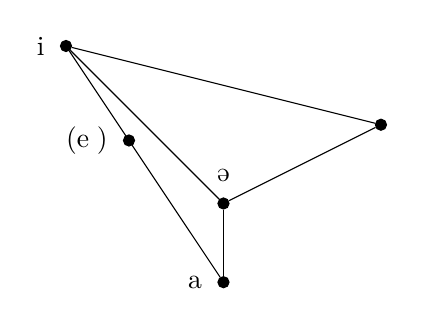
\begin{tikzpicture}
		\node[draw,fill,circle,inner sep=0pt,minimum size=4pt] (e) at (0,0) {};
		\node[draw,fill,circle,inner sep=0pt,minimum size=4pt] (i) at (-2,2) {};
		\node[draw,fill,circle,inner sep=0pt,minimum size=4pt] (o) at (2,1) {};

		\node[draw,fill,circle,inner sep=0pt,minimum size=4pt] (a) at (0,-1) {};
		\node[above=2pt of e] {ə};
		\node[left=2pt of i] {i};
		\node[right=2pt of o] {ɤ};
		\node[left=2pt of a] {a};
		\node[draw,fill,circle,inner sep=0pt,minimum size=4pt] (ee) at ($(i)!0.4!(a)$) {};
		\node[left=2pt of ee] {(eː)};

		\draw (e) -- (i) -- (o) -- (e);
		\draw (a) -- (e);
		\draw (i) -- (a);
	\end{tikzpicture}
	\caption{Mapped vowels}
\end{figure}

\subsubsection{Weak and strong vowels}
In contrast to the relatively stable /i a/, the vowel /ə/ is considered weak and pronounced with a relatively open quality and may be approximated as [ɛ]. In stressed environment, the vowel /ə/ is realized as low as [a]. On the other hand, the vowel /ɤ/ can be realized much back and acquired the roundedness to [u] when influenced by high vowel /i/.

\subsubsection{Adoption of Peninsular /e/}
Many Peninsular languages have mid-front vowel /e/. Krewi does not have this sound as a native phoneme, and speakers tend to emulate such sound more lower as [ɛː], using analogy of finer-stressed pattern of [ə]>[a], with gemination is thought as an overcompensation. Less-educated speaker and in casual speech often uses [ɪ] as the realization of the phoneme.

\subsubsection{High and low back vowel}
The back vowel phoneme /ɤ/ occupies wide range of realization, mainly influenced by the surrounding vowels and tend to assimilate the realization with the front vowels before it. Such realizations are: after /i/, it becomes

\subsection{Romanization scheme}%

Empty cells are conditions deemed impossible in Krewi.

\begin{longtblr}[
		halign = c,
		note{a} = {Only in intervocal context},
		note{b} = {Only after back coda viz. [ŋ]},
		note{c} = {Only as pausa},
	]
	{
		rowhead = 1,
		cells = {halign=c}
	}
	\toprule
	\small{archetype} & \small{lax}          & \small{tense} & \small{\_r} & \small{\_w} & \small{\_\{ɪ, ɛ, \sc{velar}\}} & \small{back}       & \small{long}   \\
	\midrule
	ɣ ⟨gh⟩            & Ø, h ⟨h⟩\TblrNote{a} & ɡː ⟨gg⟩       & x ⟨k⟩       & kʷ ⟨k⟩      & kʲ ⟨ky⟩                        & k ⟨gh⟩\TblrNote{b} &                \\
	ħ ⟨hh⟩            &                      & k ⟨hh⟩        &             &             &                                &                    &                \\
	d ⟨d⟩             & ɾ ⟨d⟩                & tsː ⟨tt⟩      & t ⟨t⟩       & tˠ ⟨t⟩      & tʃ ⟨c⟩                         &                    &              & \\
	z ⟨z⟩             &                      &               &             &             & dz ⟨z⟩                         &                    &              & \\
	ɟ ⟨j⟩             & j ⟨y⟩                & ɟʝ ⟨jj⟩       &             &             &                                &                    &              & \\
	w ⟨w⟩             &                      &               &             &             & ʝʷ ⟨zz⟩                        &                    & wː ⟨ww⟩        \\
	n ⟨n⟩             &                      & ɲː ⟨nn⟩       &             & w̃ ⟨w⟩       & ɲ ⟨ny⟩\TblrNote{c}             & ŋ ⟨ng⟩             & nː ⟨nn⟩        \\
	l ⟨l⟩             &                      &               &             &             &                                &                    & lː ⟨ll⟩        \\
	r ⟨r⟩             &                      &               &             &             &                                &                    & rː ⟨rr⟩        \\
	m ⟨m⟩             &                      &               &             &             &                                &                    & mː ⟨mm⟩        \\
	\bottomrule
\end{longtblr}


% \section{Krewi morphology}%

Morphological analysis usually entails these steps: decompose components to the morpheme-level; identifying recurrent phenomenon/elements of studied components; and then seeking generalization that lead to the most efficient and economical explanations of the formation of words.

\subsection{Decomposition of nouns}%
Underived Krewi nouns at maximum comprises of three overt morphemes. The word \emph{ralaweuy} `path, a road to follow' is realized by these morphs.

\begin{enumerate}
	\item the lexical root √\{\emph{ral-w}\}
	\item the strong patientive pattern L\textsubscript{V2}B\textsubscript{W} \{\_a\~{}eu\}
	\item noun-of-place suffix \emph{-y}
\end{enumerate}

% 
\section{Lexical Categories}
\subsection{Open classes}
There are some lexical roots that can appear in a nominal frame or in a verbal frame without any clear morphological changes. Examples are given in (\nextx).

\pex
\a \begingl
\gla ghehheye \underline{zeuraw} //
\glb own-I broom //
\glft `I own a broom' //
\endgl
\a \begingl
\gla \underline{zeuraw} jaheuw ghemalar //
\glb sweep I.\sc{agw} this.place //
\glft `I have to sweep this place' //
\endgl
\a \begingl
\gla \underline{zeuraw} zzihemer hhije méhe ralaw //
\glb sweep swing he he.\sc{attr} tail.\sc{cjt} //
\glft `His tail wags broom-likely' or `his tail wags in the manner of broom sweeping' //
\endgl
\xe

\noindent Seen above, the word \emph{zeuraw} is used nominally in (\lastx a) and verbally in (\lastx b) in the same form. Based solely on these sentences, it can be deduced that the task of determining whether a root is a noun or a verb is not always straightforward. However, establishing a distinction between Krewi nouns and verbs is relatively simple.

\subsubsection{Noun category}
One of a route to identify a noun is that by using specifier as a diagnostics. Morphologically, only nouns can be attached with \emph{mi-} `same \ldots'.\todo

\ex \vtop{\halign{%
		#\hfil&& \qquad #\hfil\cr
		\emph{zeuraw}& `broom' & \emph{mezeuraw}& `same broom' \cr
		\emph{leheye}& `person' & \emph{miléhaye}& `same person' \cr
		\emph{gharew}& `mother' & \emph{méharew}& `same mother' \cr
		\emph{lemer}& `walk' & {?\emph{milémar}}& `same journey' or `same pathway' \cr
		\emph{cenay}& `read' & \emph{*micéney} \cr
		\emph{hhejeun}& `consume' & \emph{*mihhéjeun} \cr
		\emph{nahay}& `bad' & \emph{ménahay} \cr
	}}\xe




% \section{Noun Morphology}%
In general, nouns can be a single morpheme or consist of multiple morphemes. Multiple morpheme nouns are derived from single morpheme nouns or some other form classes through three basic morphological processes, namely affixation, reduplication, and various allomorph that constitutes suppletive processes.

\subsection{Affixation}%
Affixation processes in Krewi includes prefixes, suffixes, and infixes. Many of those often multifunctional and the same configuration often bleeds into other classification, resulting many shared morphemes used in many conditions but different effects on the stem. A prime example of this is the infix \emph{-ig-} which, depending on the root, can derive root words into many conditions.

\pex
\a \vtop{\halign{%
#\hfil&& \quad #\hfil\cr
we-{\sc v} &\cr
\emph{daran} `to announce' & \emph{wedaran} `announcement' \cr
\emph{cenay} `to read' & \emph{wecanay} `reading material' \cr
\emph{ghereuy} `to want` & \emph{wahereuy} `desire` \cr
}}
\a \vtop{\halign{%
#\hfil&& \quad #\hfil\cr
we-{\sc num} &\cr
\emph{ghi} `one' & \emph{wéhi} `first' \cr
\emph{zawwar} `two' & \emph{wazawwar} `second' \cr
\emph{gherceuw} `eight' & \emph{waheurcuw} `eighth' \cr
}}
\xe


But if the verbal root is inherently patientive, the process results a habitual or frequentative verb. \todo

\ex\vtop{\halign{%
		#\hfil&& \qquad #\hfil\cr
		\emph{ghelawe} `to melt' & \emph{ghihelew} `melt easily, frequently' \cr
		\emph{jameur} `to go home' & \emph{jehameur} `go home often' \cr
	}}\xe




\section{Form I}
Form I is the base form and considered ``the dictionary form''. As a noun, the word has inherent meaning of thematic in relation with the verb. As a verb, the word appears to be intransitive or transitive.

\subsection{Examples}
Form I


\section*{Glossary}%

The romanization <e> used to represent neutral vowel.

Form I: assign neutral vowel on blanks to produce N otherwise syntactically driven otherwise. Inherently THM.

Form II: assign strong /gi/ to first slot

\dic{cenay}{o}{literary; read}
\dic{gharew}{o}{mother, host}
\dic{ghehhey}{o}{own, possess}
\dic{ghemalar}{o}{locative of this here}
\dic{ghe}{pn agt}{first person sing. with agentive color}
\dic{hhejeun}{o}{consume}
\dic{hhije}{pn}{third person sing.}
\dic{jaheuw}{pn pat}{first person sing. with patientive color}
\dic{lehēy}{o}{person, kin}
\dic{lemēr}{o}{way, road; walk}
\dic{mēhe}{pn.attr}{attributive third person sing.}
\dic{nahay}{o-adj}{badness}
\dic{ralaw}{o}{tail}
\dic{zeuraw}{o-mult.}{broom, sweepers}




\end{document}

